\documentclass[11pt]{article}
\usepackage{fullpage,titling}
\usepackage{mathtools,amssymb,amsthm}
\usepackage{bm}
\usepackage{tikz}
\usepackage{hyperref}
\usepackage{array}
\usepackage{float}
\usepackage{lstautogobble}
\usepackage[T1]{fontenc}
\usepackage{newpxtext,newpxmath}
\usepackage[activate={true,nocompatibility},final,tracking=true, kerning=true, spacing=true, factor=1100, stretch=10, shrink=10]{microtype}

\newcommand{\bu}{\bm{u}}
\newcommand{\bx}{\bm{x}}
\newcommand{\by}{\bm{y}}
\newcommand{\bz}{\bm{z}}
\newcommand{\bA}{\bm{A}}
\newcommand{\bD}{\bm{D}}
\newcommand{\bH}{\bm{H}}
\newcommand{\bI}{\bm{I}}
\newcommand{\bJ}{\bm{J}}
\newcommand{\bX}{\bm{X}}
\newcommand{\bY}{\bm{Y}}
\newcommand{\bbeta}{\bm{\beta}}
\newcommand{\btheta}{\bm{\theta}}

\newcommand{\bbr}{\mathbb{R}} 
\newcommand{\bbq}{\mathbb{Q}}
\newcommand{\bbn}{\mathbb{N}}

\newcommand{\semicol}{\nobreak\mskip2mu\mathpunct{}\nonscript\mkern-\thinmuskip{;}\mskip6muplus1mu\relax}

\DeclareMathOperator{\sign}{sgn}
\DeclareMathOperator{\prox}{prox}
\DeclareMathOperator{\diag}{diag}
\DeclareMathOperator{\bprox}{\mathbf{prox}}
\DeclareMathOperator*{\argmin}{arg\,min}

\newcommand{\refthm}[2]{#1~#2}

\title{Notes on Approximate Leave-One-Out for Elastic Net}
\author{Linyun He \and Wanchao Qin \and Peng Xu \and Yuze Zhou}

\begin{document}
\maketitle

\section{ALO for Elastic Net, Approximation in the Primal Domain}
Recall the objective function for the elastic net problem: \[\min_{\bbeta}\frac{1}{2}\sum_{j=1}^{n}(\bx_j^\top\bbeta-y_j)^2+\lambda\left(\alpha\|\bbeta\|_1+\frac{1-\alpha}{2}\|\bbeta\|_2^2\right).\] Let \(A=\{i:\beta_i\not\in K,i=1,\dotsc,p\}\) be the active set, we have \[\dot{\ell}(\bx_j^\top\bbeta\semicol y_j)=\bx_j^\top\bbeta-y_j,\qquad\ddot{\ell}(\bx_j^\top\bbeta\semicol y_j)=1,\qquad\nabla^2 R(\hat{\bbeta}_A)=(1-\alpha)\lambda\bI_{A,A}.\] Thus, \refthm{Eqn.}{31} reduces to \[\bH=\bX_{\cdot,A}\left[\bX_{\cdot,A}^\top\bX_{\cdot,A}+\left(1-\alpha\right)\lambda\bI_{A,A}\right]^{-1}\bX_{\cdot,A}^\top.\] By augmenting \(\bX\) with an extra column of \(1\)s, adding the intercept back to the model is straightforward, as \refthm{Eqn.}{31} now becomes \[\bm{H}=\left[\bm{1}_n,\bm{X}_{\cdot, A}\right]\left\{\left[\bm{1}_n,\bm{X}_{\cdot, A}\right]^\top\bm{D}\left[\bm{1}_n,\bm{X}_{\cdot, A}\right]+\nabla^2R\left(\hat{\beta}_0,\hat{\bm{\beta}}_A\right)\right\}^{-1}\left[\bm{1}_n,\bm{X}_{\cdot, A}\right]^\top,\] where \[\bm{D}=\diag\left[\ddot{\ell}\left(\hat{\beta}_0+\bm{x}_j^\top\hat{\bm{\beta}};y_j\right)\right]_{j\in A}=\bI_{A,A},\qquad\nabla^2R\left(\hat{\beta}_0,\hat{\bm{\beta}}_A\right)=\begin{bmatrix}
0 & 0 & \dots & 0 \\
0 & (1-\alpha)\lambda & \dots & 0\\
\vdots & \vdots & \ddots & \vdots\\
0 & 0 & \dots & (1-\alpha)\lambda \\
\end{bmatrix}.\] Therefore, the ALO update is \[\begin{bmatrix}
1 & \bm{x}_i^\top\end{bmatrix}
\begin{bmatrix}
\tilde{\beta}_0^{\setminus i} \\
\tilde{\bm{\beta}}^{\setminus i}\end{bmatrix}=(\hat{\beta}_0+\bm{x}_i^\top\hat{\bm{\beta}})+\frac{\bH_{ii}}{1-\bH_{ii}\ddot{\ell}\left(\hat{\beta}_0+\bm{x}_i^\top\hat{\bm{\beta}};y_i\right)}\dot{\ell}\left(\hat{\beta}_0+\bm{x}_i^\top\hat{\bm{\beta}};y_i\right)\]

\section{ALO for Elastic Net, Approximation in the Dual Domain}
The original problem for elastic net is to solve for $\hat{\bbeta}$ such that: \[\hat{\bbeta}=\argmin\limits_{\bbeta}\left(\frac{1}{2}||\by-\bX\bbeta||_{2}^{2} + \lambda_{1}||\bbeta||_{1}+\lambda_{2}||\bbeta||_{2}^{2}\right).\] By adding the Lagrangian, we get the formulation of $L$: \[L = \frac{1}{2}||\by-\bz||_{2}^{2} + \lambda_{1}||\bbeta||_{1}+\lambda_{2}||\bbeta||_{2}^{2}+u^{\top}(\bz-\bX\bbeta).\] The original problem is solving the primal of the Lagrangian such that $p^{*} = \min\limits_{\bbeta,\bz}\max\limits_{\bu}L$ and the dual formulation $d^{*} = \max\limits_{\bu}\min\limits_{\bbeta,\bz}L$, to minimize over $\bz$: \[\frac{\partial L}{\partial \bz} = \bz -\by +\bu = \bm{0}\implies \by = \bu + \bz.\] Since $\bbeta$ is penalized element-wisely, we can minimize over $\bbeta$ by minimizing over each $\bbeta_{i}$, that is, we have to minimize $\lambda_{1}|\beta_{i}| + \lambda_{2}\beta_{i}^{2} - \bu^{\top}\bX_{i}\bbeta$ for each dimension of $\bbeta$, where $\bX_{i}$ denotes the $i$th column of $\bX$, therefore: \[\min\limits_{\bbeta}\left(\lambda_{1}|\beta_{i}| + \lambda_{2}\beta_{i}^{2} - \bu^{\top}\bX_{i}\bbeta\right)=\begin{dcases}
0 & |\bu^{\top}\bX_{i}| \leq \lambda_{1},\\
-\frac{(\lambda_{1}-|\bu^{\top}\bX_{i}|)^{2}}{4\lambda_{2}} & |\bu^{\top}\bX_{i}| > \lambda_{1}.
\end{dcases}\] By taking all the above to the Lagrangian, we could obtain the dual problem $d^{*}$ as: \[d^{*} = \min\limits_{\bu}\frac{1}{2}||\by-\bu||_{2}^{2} + \sum_{j: |\bX_{j}^{\top}\bu| > \lambda_{1}}\frac{(\lambda_{1}-|\bu^{\top}\bX_{i}|)^{2}}{4\lambda_{2}}.\] The minimizer $\hat{\bu}$ could also be obtained from the dual problem through a proximal approach: \[\hat{\bu} = \bprox_{R}(y),\qquad\quad R(\bu) = \sum_{j:|\bX_{j}^{\top}\bu| > \lambda_{1}}\frac{(\lambda_{1}-|\bu^{\top}\bX_{i}|)^{2}}{4\lambda_{2}}.\]

By replacing the full data problem $\by$ with $\by_{\alpha} = \by + (y_{i}^{\setminus i}-y_{i})e_{i}$, where $y_{i}^{\setminus i}$ is the true LOO estimator and $e_{i}$ is the $i$-th standard vector, and let $\bu^{\setminus i} = \bprox_{R}(\by_{\alpha})$, we have:
\begin{align*}
0 &= e_{i}^{\top}\bu^{\setminus i}\\
& = e_{i}^{\top}\bprox_{R}(\by_{\alpha})\\
& \approx e_{i}^{\top}[\bprox_{R}(\by)+\bJ_{R}(\by)(\by_{\alpha}-\by)]\\
& \approx \hat{u}_{i} + \bJ_{ii}(y_{i}^{\setminus i}-y_{i}).
\end{align*} Here $\bJ_{R}(\by)$ denotes the Jacobian matrix of the proximal operator at $\by$, thus the ALO estimator $\tilde{y}_{i}$ is obtained as \[\tilde{y}_{i} = y_{i} - \frac{\hat{\bu}_{i}}{\bJ_{ii}}.\] The Jacobian could locally be obtained as:\[\bJ_{R}(\by)= (\bI+\nabla^{2}R(\bprox_{R}(\by)))^{-1}= (\bI + \nabla^{2}R(\hat{\bu}))^{-1}= \left(\bI + \frac{1}{2\lambda_{2}}\bX_{E}\bX_{E}^{\top}\right)^{-1}\] for $E = \{j:|\bX_{j}^{\top}\bu|>\lambda_{1}\}$.

\section{ALO for Elastic Net, Approximation with Proximal Formulation}
For the elastic net problem, the proximal mapping is known to be \[\bprox_R\left(\bz\right)=\gamma\sign(\bz)\odot(|\bz|-\lambda\bm{1}_p)_+,\qquad\gamma=\frac{1}{1+(1-\alpha)\lambda}.\] Let \(E\) be the active set, if \(z_i\in E\), then \[\frac{\partial}{\partial z_i}\gamma\sign(z_i)(|z_i|-\lambda)_+=\gamma.\] Plug in \(\bz=\hat{\bbeta}-\sum_{j=1}^{n}\dot{\ell}(\bx_j^\top\hat{\bbeta}\semicol y_j)\bx_j\), \refthm{Eqn.}{46} thus reduce to \[\bH=\gamma\bX_{\cdot,E}\left[\gamma\bX_{\cdot,E}^\top\bX_{\cdot,E}+\left(1-\gamma\right)\bI_{E,E}\right]^{-1}\bX_{\cdot,E}^\top.\]
Bringing back the intercept term is straightforward as well. Noted that \[\begin{bmatrix}
\hat{\bbeta}_0^{\setminus i} \\
\hat{\bm{\bbeta}}^{\setminus i}\end{bmatrix}=
\bprox_{R}\left(\bz\right),\qquad\bz=\begin{bmatrix}
\hat{\bbeta}_0^{\setminus i} \\
\hat{\bm{\bbeta}}^{\setminus i}\end{bmatrix}-
\sum_{j\neq i}\begin{bmatrix}
1 \\
\bm{x}_j\end{bmatrix}
\dot{\ell}\left(\hat{\bbeta}_0^{\setminus i}+\bm{x}_j^\top\hat{\bm{\bbeta}}^{\setminus i};y_j\right).\] Hence, from the first-order condition \(\sum_{j\neq i}\dot{\ell}\left(\hat{\bbeta}_0^{\setminus i}+\bm{x}_j^\top\hat{\bm{\bbeta}}^{\setminus i};y_j\right)=0\), we can derive that \[\bm{J}_{E,E}=
\left[\bm{J}(\bm{u})\right]_{E,E}=
\begin{bmatrix}
1 & 0 & 0 & \dots & 0\\
0 & (1-\alpha)\lambda & 0 & \dots & 0\\
0 & 0 & (1-\alpha)\lambda & \dots & 0\\
\vdots & \vdots & \vdots & \ddots & \vdots\\
0 & 0 & 0 & 0 & (1-\alpha)\lambda\\
\end{bmatrix}^{-1}.\] The ALO formula is then immediate by \refthm{Thm.}{5.1}.

\section{ALO for LASSO, with Intercept through Generalized LASSO}
For the generalized LASSO problem \[\min\limits_{\bbeta}\frac{1}{2}||\by-\bX\bbeta||+\lambda||\bD\bbeta||_{1},\] the dual problem is derived as: \[\min\limits_{\bu}\frac{1}{2}||\by-\btheta||_{2}^{2},\qquad\theta\in \{\bX^{\top}\btheta = \bD^{\top}bu, ||\bu||_{\infty} \leq \lambda\}.\] The dual problem could be written in a proximal approach, such that: \[\hat{u} = \bprox_{R}(\by),\qquad R(\bu) =\begin{dcases}
0 & \btheta \in \{\bX^{\top}\btheta = \bD^{\top}\bu, ||\bu||_{\infty} \leq \lambda\},\\
\infty & \text{otherwise.}
\end{dcases}\] Denote $\bJ$ as the Jacobian of the proximal operator at the full data problem $\by$, then the ALO estimator could be obtained as: \[\by^{\setminus i} = \by_{i} - \frac{\hat{\bu}_{i}}{\bJ_{ii}}.\] For the case of LASSO with an intercept, we could expand the $\bX$ with a column of ones in the first column, expand $\bbeta$ with another dimension and choose $\bD = [\bm{0}, \bI]$. Let \(E\coloneqq\{j:|\bX_{j}^{\top}\theta| = \lambda \}\) denote the active set. The Jacobian is locally given as the projection onto the orthogonal complement of the span of $\bX_{E}$ and the vector of ones. Further denote $\tilde{\bX}_{E} = [\textbf{1}, \bX_{E}]$, then the Jacobian is given as $\bI - \tilde{\bX_{E}}(\tilde{\bX}_{E}^{\top}\tilde{\bX}_{E})\tilde{\bX}_{E}^{\top}$.

\section{Usage of ALO formulae with \texttt{glmnet} package}
The \verb|glmnet| package scales the elastic net loss function by a factor of \(1/n\), so the ALO formulae must be adjusted accordingly, e.g. for the proximal one, we instead have: \[\tilde{\by}_j^{\setminus i}=\hat{\by}_j+\frac{\bH_{ii}(\hat{\by}_j-\by_j)}{n-\bH_{ii}},\qquad\bH=\gamma\bX_{\cdot,E}\left[\frac{\gamma}{n}\bX_{\cdot,E}^\top\bX_{\cdot,E}+\left(1-\gamma\right)\bI_{E,E}\right]^{-1}\bX_{\cdot,E}^\top.\]

Furthermore, \verb|glmnet| implicitly ``standardizes \(y\) to have unit variance before computing its \(\lambda\) sequence (and then unstandardizes the resulting coefficients)''. So to get comparable result, it is necessary to rescale \(\by\) by the MLE \(\hat{\sigma}_y\) before fitting the model. \autoref{fig:elsnet} shows the comparison of the ALO and LOO for different \(\alpha\)s. Without standardizing \(\by\) first, a growing discrepancy between the two curves can be observed as \(\alpha\to0\).
	\begin{figure}[!htbp]
		\centering
		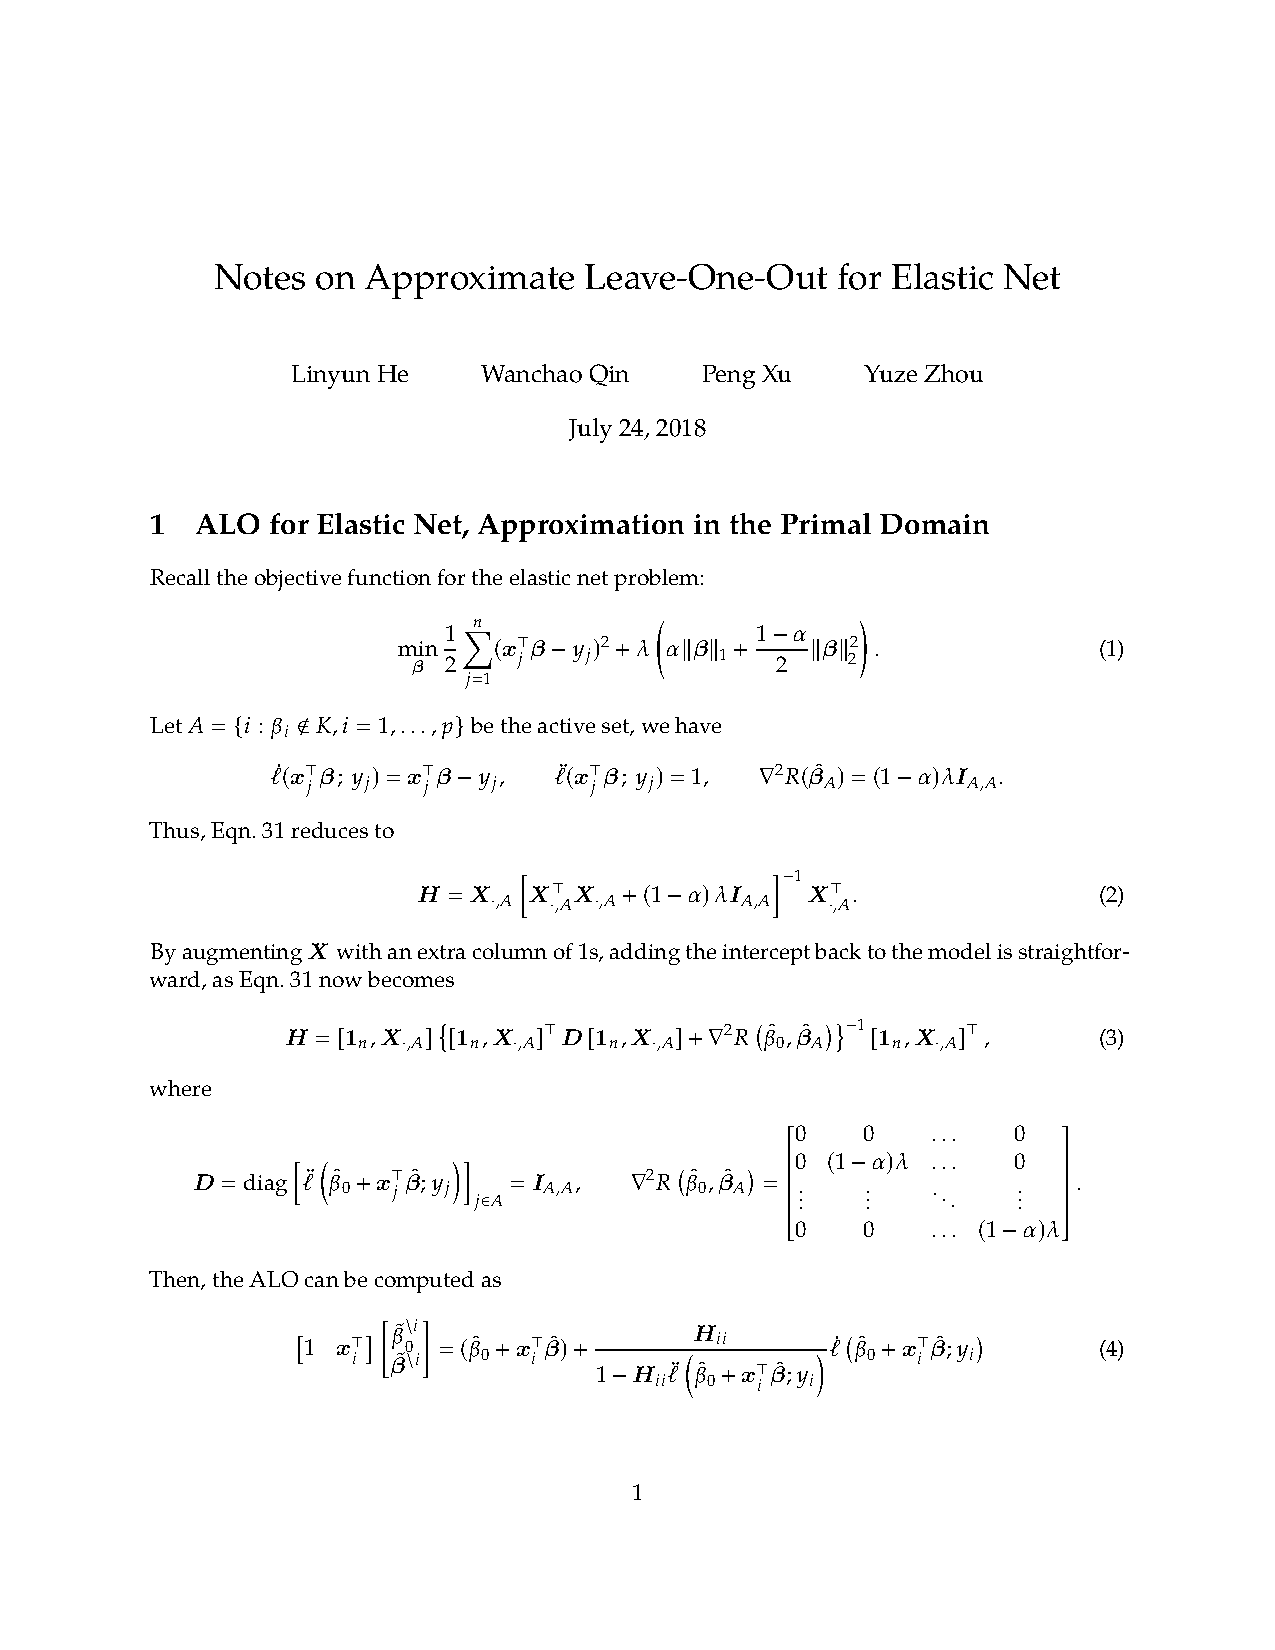
\includegraphics[width=\textwidth,height=\textheight,keepaspectratio]{elsnet.png}
		\caption{ALO vs. LOO for Elastic Net. \label{fig:elsnet}}
	\end{figure}
\end{document}